\documentclass[presentation, aspectratio=1610]{beamer}
\usepackage[utf8]{inputenc}
\usepackage[TS1,T1]{fontenc}
\usepackage[english]{babel}
\usepackage{amsmath}
\usepackage{graphicx}
\usepackage{float}
\usepackage{amssymb}
\usepackage{hyperref}
\usepackage[round]{natbib}
\usepackage[normalem]{ulem}
\usepackage{listings}
\usepackage{lstautogobble}
\usepackage{mdframed}
\usepackage{showexpl}
\lstset{explpreset = {vsep=6pt,pos=r},
		basicstyle=\scriptsize\ttfamily,
		numbers=left,
		breaklines=true,
		breakindent=0pt,
		tab=\rightarrowfill,
		backgroundcolor =\color{lightgray},
		xleftmargin = 1cm,
		framexleftmargin = 1em,
		rframe={}
}
\usepackage{caption}
\captionsetup{font=scriptsize,labelfont=scriptsize}
\beamertemplatenavigationsymbolsempty
\usecolortheme{beaver}
\setbeamertemplate{footline}[frame number]
\title[Introduction to \LaTeX]{A short introduction to \LaTeX}
\author[J.Feldbauer, C. Ordóñez]{Johannes Feldbauer \& César Ordóñez}
\date{\today}

\bibliographystyle{apalike}

\begin{document}
	\maketitle

	\begin{frame}{Table of contents}
	\begin{minipage}[c][.75\textheight]{0.6\textwidth}
		\tableofcontents
	\end{minipage}
	\begin{minipage}{0.25\textwidth}
		%\includegraphics[width=\textwidth]{intro.png}
	\end{minipage}
	\end{frame}

	\section{What is \LaTeX ?}
	\begin{frame}{What is \LaTeX ?}
		\begin{itemize}[<+->]
			\item It is a typesetting system originally written by Lesslie Lamport, which uses \TeX{}  as its formatting engine
			\item \TeX{} is a computer program for typesetting text and mathematical formulae created by Donald E. Knuth
			\item Main idea: split writing and formating of the document
			\item Special commands give the software information about structure of the document
			\item The document is written as a \texttt{ASCII} text-file and translated by the program into a post script document or a pdf
		\end{itemize}
	\vfill
	\begin{block}{}
		{\footnotesize Most of this introduction is taken from: \textit{The Not So Short Introduction to \LaTeXe} by
			Tobias Oetiker, Hubert Partl, Irene Hyna and Elisabeth Schlegl (\url{https://tobi.oetiker.ch/lshort/lshort.pdf})}
	\end{block}
	\end{frame}

	\begin{frame}{Example - article}
		Write an article or paper using e.g. \texttt{\textbackslash{}documentclass\{article\}}. Also many journals and publishers
		provide \LaTeX{} templates.
		\begin{figure}
			\centering
			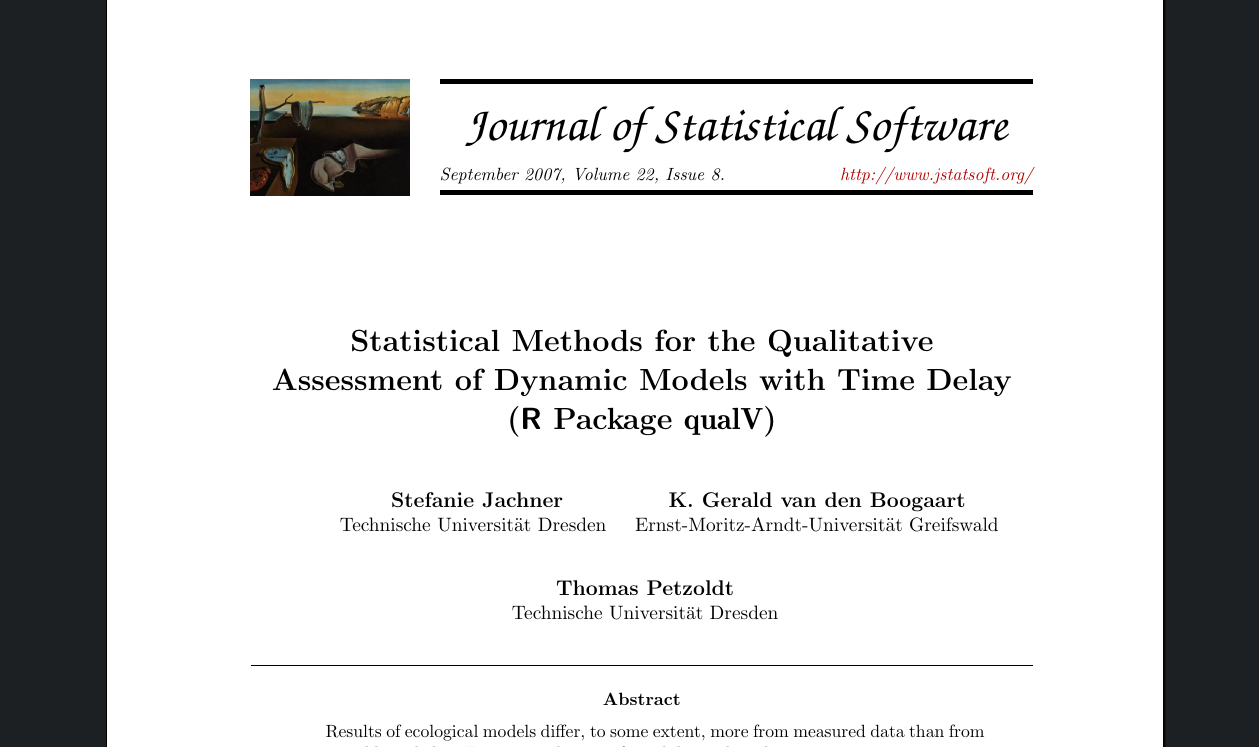
\includegraphics[width=.85\linewidth]{article_example}
		\end{figure}
	\end{frame}

	\begin{frame}{Example - book}
		Write a book (or your dissertation) using e.g. \texttt{\textbackslash{}documentclass\{book\}}
		\begin{figure}
			\centering
			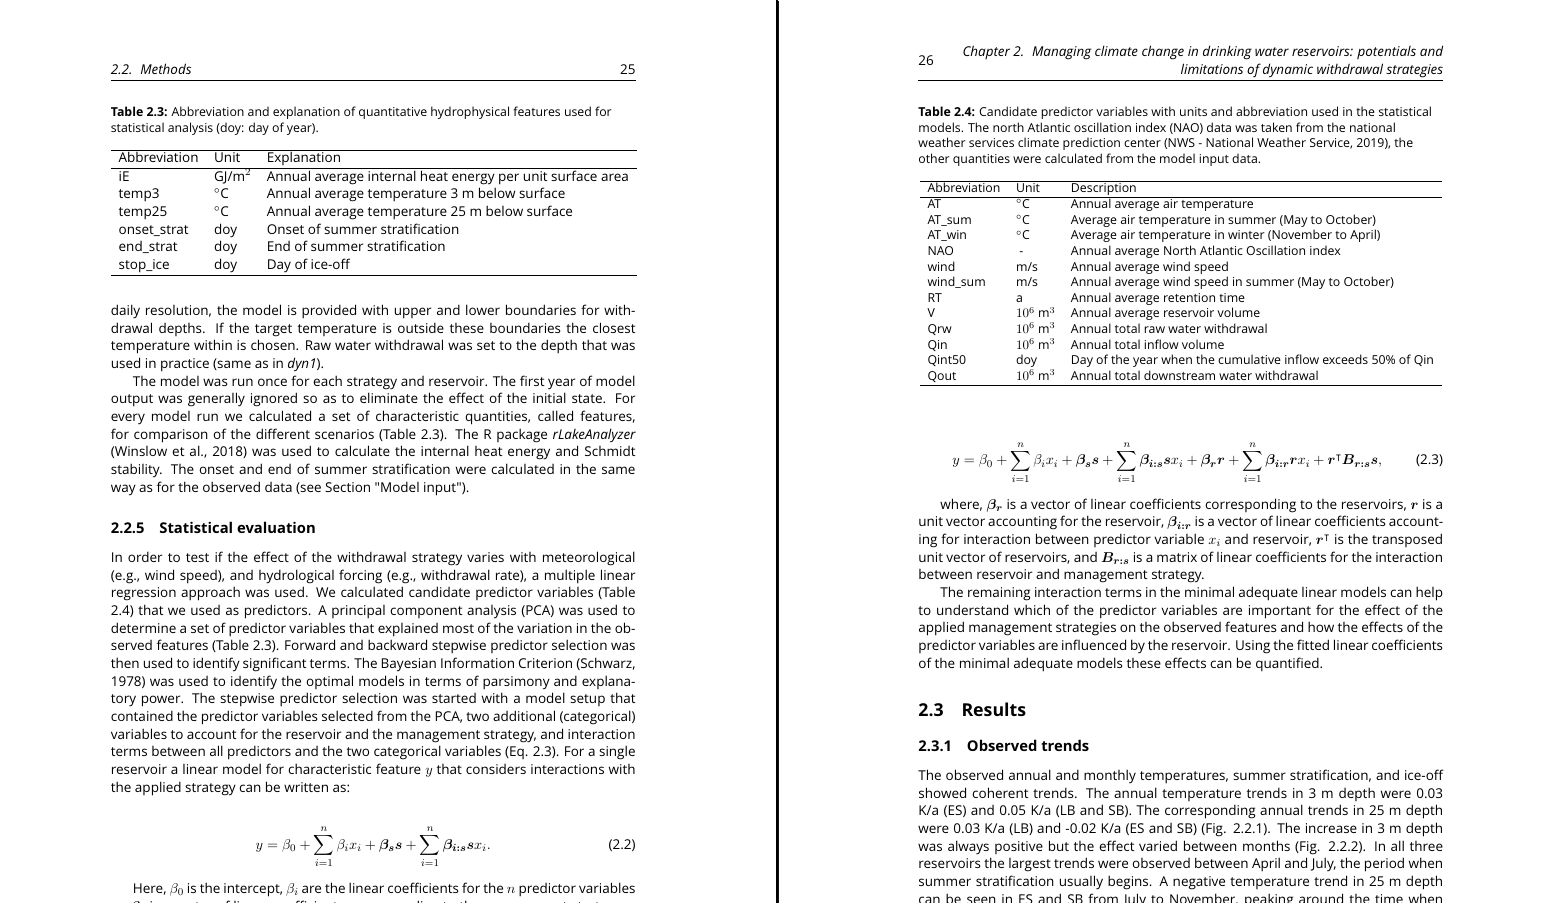
\includegraphics[width=.85\linewidth]{book_example}
		\end{figure}
	\end{frame}

	\begin{frame}{Example - CV}
		Create your curriculum vitae in \LaTeX{} using e.g. \texttt{\textbackslash{}documentclass\{moderncv\}}
		\begin{figure}
			\centering
			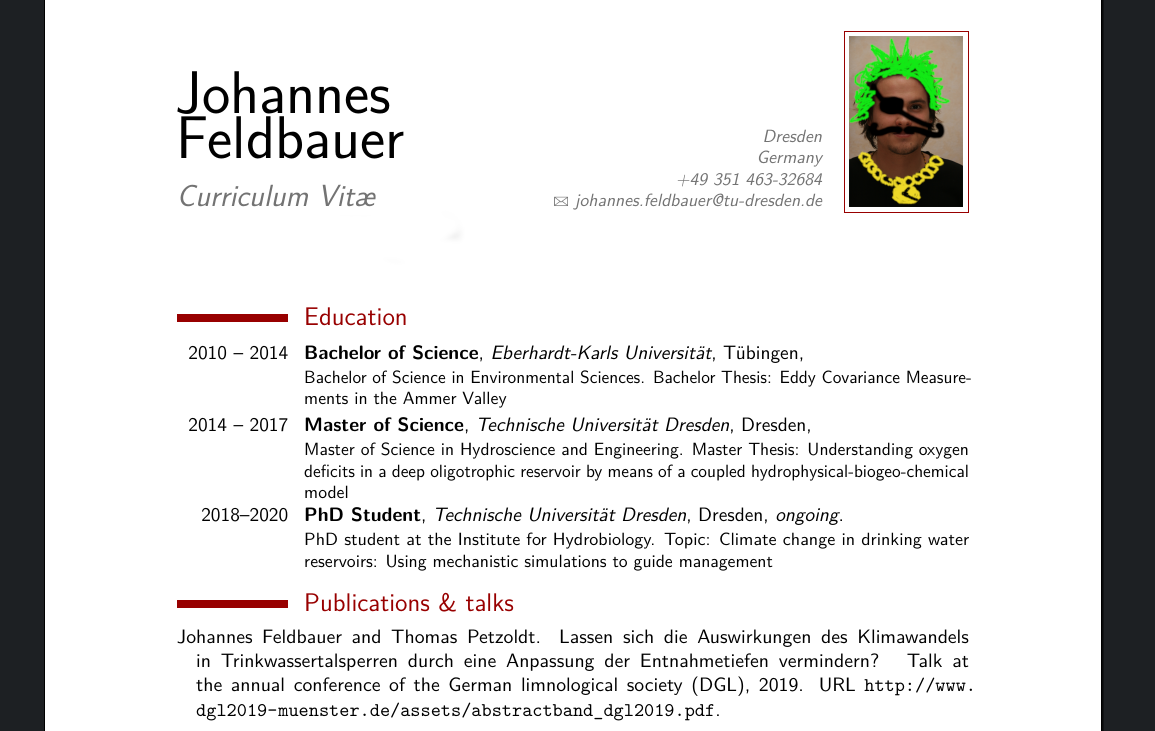
\includegraphics[width=.85\linewidth]{CV_example}
		\end{figure}
	\end{frame}

	\section{Why (or why not) use \LaTeX ?}
	\begin{frame}{Why (or why not) use \LaTeX ?}
	\begin{columns}[t]
		\column{0.5\textwidth}
		{\large \color{green}\textbf{Pros}}
		\begin{itemize}
			\item [\color{green}\textbf{+}] Produces beautiful high quality documents
			\item [\color{green}\textbf{+}] Especially nice for equations
			\item [\color{green}\textbf{+}] Open Source with lots of add-ons
			\item [\color{green}\textbf{+}] Only text files (good for version control and
			collaboration)
			\item [\color{green}\textbf{+}] Can be included in automatization
			\item[\color{green}\textbf{+}] \color{gray} Easy to change layout of whole document
			\item[\color{green}\textbf{+}] Automated TOC and others
			\item[\color{green}\textbf{+}] All the cool kids use it ;-)
		\end{itemize}
	\pause
		\column{0.5\textwidth}
			{\large \color{red}\textbf{Cons}}
		\begin{itemize}
			\item [\color{red}\textbf{-}] Can be confusing (no WYSIWYG - what you see is what you get)
			\item [\color{red}\textbf{-}] In the beginning hard to learn (and most possibly frustrating)
			\item [\color{red}\textbf{-}] Not everybody knows it (collaboration)
			\item [\color{red}\textbf{-}] The layout is (mostly) pre-defined, design of whole new
			layout is challenging
		\end{itemize}
	\end{columns}
	\end{frame}

	\section{Basic Concept}

	\begin{frame}[fragile]{Structure of a LaTeX document}
		The source code of a \LaTeX{} document is a plain text file with ending \textit{.tex}.
		\begin{lstlisting}[showspaces = false,showtabs = false,basicstyle=\tiny\ttfamily]
\documentclass{article}   % the first command must set the class of the document

% everything before "\begin{document}" is called preamble

\usepackage{packagename}  % additional packages are included using this command
\bibliographystyle{style} % set the style of citations

\author{A. Uthor}         % name of the author

\begin{document}

	\maketitle        % create a title
	\tableofcontents  % create a table of content from the given sections, etc
	\listoffigures    % create a table of figures
	\listoftables     % create a table of tables

	\section{Introduction}

	Some text about the figure \ref{key}. And some more Text without any content but with source cited \citep{bibid}. Now the text is at the end.

	\begin{figure}
		\centering
		\includegraphics[width=\textwidth]{imagefile}
		\caption[short text]{text}\label{key}
	\end{figure}

	\bibliography{bib_file}   % name of the biblography file

\end{document}
		\end{lstlisting}
	\end{frame}

	\begin{frame}{Documentclass}

		Every input file (e.g. \textit{main.tex}) must begin (exept for comments) with the command:

		\begin{block}{}\centering
			\texttt{\textbackslash{}documentclass[options]\{class\}}
		\end{block}
		\vspace{1em}
		which is declaring the document class of the file, e.g. article, book, or beamer. Usually this is followed by the \textit{preamble}
		in which all used packages are loaded and settings for the whole document can be changed.

		The main text body is within the document \textit{environment}:
		\begin{block}{}\centering
			\texttt{\textbackslash{}begin\{document\}}\\\noindent
			...\\ \noindent
			\texttt{\textbackslash{}end\{document\}\hspace{1em}}

		\end{block}
	\end{frame}


	\begin{frame}[fragile]{The preamble}
		The area between \texttt{\textbackslash{}documentclass} and \texttt{\textbackslash{}begin\{document\}} is called the
		\textit{preamble}. Here the used packages are loaded and global settings can be changed
		\begin{lstlisting}[showspaces = false,showtabs = false,basicstyle=\scriptsize\ttfamily,language=tex]
\documentclass{beamer}
% begin preamble
\usepackage{abstract}
\usepackage{float}
\usepackage{amssymb}
\usepackage{hyperref}
\usepackage[round]{natbib}

\title{good read}
\author{Anna und Arthur}

\beamertemplatenavigationsymbolsempty
\usecolortheme{beaver}
\setbeamertemplate{footline}[frame number]
% begin text body
\begin{document}
			\end{lstlisting}

		\end{frame}

	\section{Important commands \& examples}

	\begin{frame}{\LaTeX{} Commands}
	\LaTeX{} Commands are case sensitive, and take one of the following two formats:
	\begin{enumerate}[<+->]
		\item They start with a backslash \textbf{\textbackslash{}} and then have a name consisting of letters only; command names are
		terminated by a space, a number or any other "non-letter"
		\item They consist of a backslash and exactly one non-letter e.g. \texttt{\textbackslash \&}
		\item \LaTeX{} Ignores whitespace after commands; to get a space after a command empty parameters \{ \} and a blank after the
		command are used e.g. \texttt{\textbackslash LaTeX\{\}}
	\end{enumerate}
	\begin{block}{}\centering
	\texttt{\textbf{\textbackslash command}[optional parameter]\{parameter\}}
	\end{block}
	\end{frame}
	\begin{frame}{Commands \& special characters}
	\begin{block}{Characters with special meaning:}
		\centering
		\# \$ \% \^{} \& \_ \{ \} \~{} \textbackslash
	\end{block}
	\pause
	\begin{block}{Groups and environments:}
		\begin{tabular}{rl}
			Group:& in between \{ \} \\
			Environment:&  \texttt{\textbackslash begin\{environment\}}\\
			& \texttt{\textbackslash  end\{environment\}}
		\end{tabular}
	\end{block}
	\pause
	\begin{block}{Comments:}
		Everything following \texttt{\%} or in the \texttt{comment} environment from the \texttt{verbatim} package
	\end{block}
	\end{frame}

	\begin{frame}{Floating Bodies}
		\begin{itemize}[<+->]
			\item Tables or figures, which cannot be broken across pages are placed by \LaTeX{} in a way that not too many empty
			pages are created
			\item For floating environments so called \textit{placement specifier} can be given in the optional arguments
			\item Possible \textit{placement specifiers} are: \texttt{htbp!}
			\item If nothing is given the standard classes will assume \texttt{[tbp]}
			\item If a float cannot be placed on the current page it is deferred to a queue (first in first out)
			\item Using \texttt{\textbackslash{}caption[short caption]\{long caption\}} a caption for the floating body can be created
		\end{itemize}
	\end{frame}

	\begin{frame}[fragile]{Tables}
		Creating tables in \LaTeX{} is usually done using the \texttt{tabular} environment \pause
		\begin{LTXexample}[pos=b,firstline=2,basicstyle=\tiny\ttfamily,xleftmargin = 0cm,framexleftmargin = 0em,numbers=none]
			\centering
			\begin{table}
				\caption{This is the caption of the table.}
				\begin{tabular}{lcr}
					\hline
					Variable & Date & Value \\ \hline
					Temp & 2000-12-01 & 0.7 \\
					Temp & 2000-12-02 & 1.3 \\
					\vdots & \vdots & \vdots \\\hline
				\end{tabular}
			\end{table}
		\end{LTXexample}

	\end{frame}

	\begin{frame}[fragile]{Images}
		Including images in \LaTeX{} is usually done using the \texttt{includegraphics} command
		\begin{LTXexample}[pos=b,basicstyle=\tiny\ttfamily,xleftmargin = 0cm,framexleftmargin = 0em,numbers=none]
			\begin{figure}
				\centering
				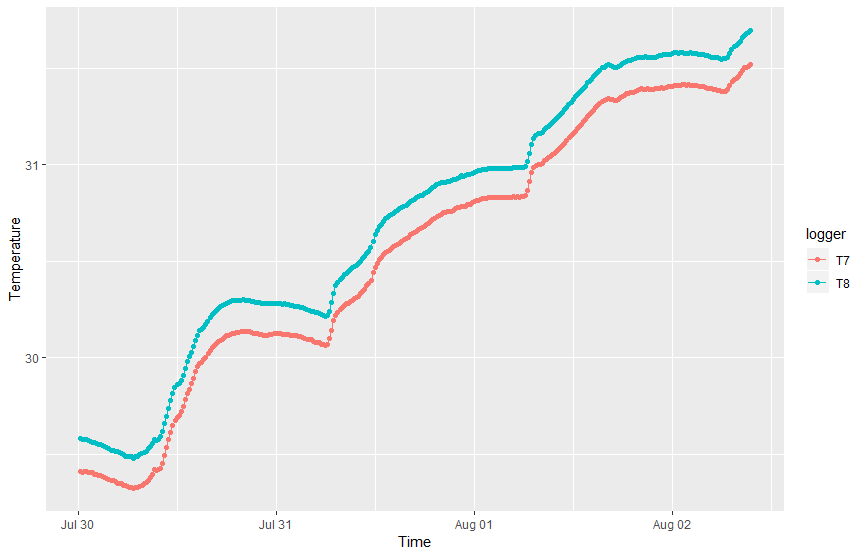
\includegraphics[width=.5\linewidth]{example_figure}
				\caption{This is the figure caption.}
			\end{figure}
		\end{LTXexample}
	\end{frame}

	\begin{frame}[fragile]{Math mode}
		\LaTeX{} can produce beautiful equations using e.g. the \texttt{equation} or the \texttt{align} environment \pause
		\begin{LTXexample}[pos=b,firstline=3,basicstyle=\tiny\ttfamily,xleftmargin = 0cm,framexleftmargin = 0em,numbers=none]
			\abovedisplayskip0pt
			\footnotesize
\begin{align}
	y &= c_1 \cdot \sin \left( \frac{2 \cdot \pi \cdot (x + c_2)}{365.25} \right) \\
	x(t) &= \int_{t=0}^{\inf} \log \left( \frac{1}{t} \cdot x \right) \text{d}t \\
	\frac{\partial x}{\partial t} &= \frac{1}{\rho} \sqrt[3]{x} + \vec{a}
\end{align}
		\end{LTXexample}
	\end{frame}

	\begin{frame}[fragile]{Referencing}
	\begin{itemize}\scriptsize
		\item In \LaTeX{} it is possible to create cross references within the document \pause
		\item \texttt{\textbackslash{}label\{key\}} is used to label items (e.g. equations, figures, tables, sections,...)
		\item \texttt{\textbackslash{}ref\{key\}} is used to refer to their number
		\item \texttt{\textbackslash{}pageref\{key\}} refers to the page number of the labeled item
		\item \texttt{\textbackslash{}cref\{key\}} refers to the type of the item (if known)
	\end{itemize}
	\pause
	\begin{LTXexample}[firstline=2,pos=r,xleftmargin = 0cm,framexleftmargin = 0em,numbers=none,rframe=single,basicstyle=\tiny\ttfamily]
\scriptsize
this is an example equation:

\begin{equation}\label{eq:hail}
	2 + 2 \approx 5
\end{equation}

now we can refer to equation
\ref{eq:hail} on page \pageref{eq:hail}
	\end{LTXexample}

\end{frame}

	\begin{frame}[fragile]{Citations}
		Creating citations is very simple in \LaTeX{} but we need to create a separate bibliography-file (a plain text file ending in \textit{.bib})
		containing the literature information
		\begin{lstlisting}[pos=b,xleftmargin = 0cm,framexleftmargin = 0em,numbers=none,rframe=single,language=tex]
Some Text that needs citation \citep{wilhelm_2008}.
Another study by \citet{huisman_2004} showed something else.

\bibliography{bib_file}
		\end{lstlisting}

		\begin{mdframed}[linecolor=black,fontcolor=black]
			\scriptsize
			Some Text with a statement that needs citation \citep{wilhelm_2008}. Another study by \citet{huisman_2004} showed something else.

			\vspace{1em}
			\textbf{Bibliography}
			\bibliography{bib_file}
		\end{mdframed}
	\end{frame}

	\begin{frame}[fragile]{Citations}
		The corresponding bibliography file \textit{bib\_file.bib} looks like this
		\begin{lstlisting}[pos=b,xleftmargin = 0cm,framexleftmargin = 0em,numbers=none,rframe=single,basicstyle=\tiny]
@article{huisman_2004,
	title = {Changes in turbulent mixing shift competition for light between phytoplankton species},
	volume = {85},
	number = {11},
	journal = {Ecology},
	author = {Huisman, Jef and Sharples, Jonathan and Stroom, Jasper M. and Visser, Petra M. and Kardinaal, W. Edwin A. and Verspagen, Jolanda MH and Sommeijer, Ben},
	year = {2004},
	pages = {2960--2970},
	doi = {10.1890/03-0763}
}

@article{wilhelm_2008,
	title = {Impact of summer warming on the thermal characteristics of a polymictic lake and consequences for oxygen, nutrients and phytoplankton},
	volume = {53},
	issn = {1365-2427},
	doi = {10.1111/j.1365-2427.2007.01887.x},
	language = {en},
	number = {2},
	journal = {Freshwater Biology},
	author = {Wilhelm, Susann and Adrian, Rita},
	month = feb,
	year = {2008},
	pages = {226--237}
}
		\end{lstlisting}

	\end{frame}


	\begin{frame}{Whitespace and empty lines}
	\begin{itemize}
		\item Whitespace characters, such as \textit{space} \textvisiblespace{} or \textit{tab} $\leftrightarrows$, are treated uniformly as space
		\item Several whitespace characters are treated as one \textit{space}
		\item Whitespace at the start of a line is generally ignored
		\item A single line break is treated as whitespace
		\item An empty line between two lines of text defines the end of a paragraph
		\item Several empty lines are treated the same as one empty line
	\end{itemize}
\end{frame}

	\begin{frame}[fragile]{Whitespace example}
		\textbf{this:}
		\begin{LTXexample}[showspaces = true,showtabs = true,rframe=simple]
			test test test

			test
		\end{LTXexample}

		\textbf{is the same as this:}

		\begin{LTXexample}[	showspaces = true,showtabs = true,rframe=simple]
			test
			test    test


			test
		\end{LTXexample}
	\end{frame}


	\begin{frame}{Material}

    good sources for help are:
    \vspace{1em}

        \begin{itemize}
            \item google and especially stackexchange \url{https://tex.stackexchange.com/}
            \item The Not So Short Introduction to \LaTeXe{} by Tobias Oetiker, Hubert Partl, Irene Hyna and Elisabeth Schlegl \url{https://tobi.oetiker.ch/lshort/lshort.pdf}
            \item \LaTeXe{} cheat sheet: \url{https://wch.github.io/latexsheet/}
            \item \LaTeX{} for complete Novices by Nicola L. C. Talbot \url{http://www.dickimaw-books.com/latex/novices/}
        \end{itemize}
    \end{frame}


	\begin{frame}{Questions?}
		\begin{columns}[c]
			\column{0.6\textwidth}

			\Large{\textbf{\textcolor{gray}{lets try it out together}}}

			\column{0.3\textwidth}

		\end{columns}
	\end{frame}


\end{document}
